%\usepackage{tikz}
%\usetikzlibrary{positioning}
%\usepackage{endnotes}
%\usepackage[ruled,vlined]{algorithm2e}
%\usepackage{caption}
%\usepackage{comment}
%\usepackage{times}
%\begin{document}

\chapter{HAWK -- Hybrid Question Answering using Linked Data}



Structured data offers the possibility to truly 
The 
document web:
petabytes of data , unstructured -> not machine readable
hard to extract semantics

Linked data web
highly structured
semantic information
easier to answer information need

however there is a INFORMATION MISMATCH 

for example this information comes from the document web
the other information comes from the DBpedia

hence we aim to develop a framework to develop to combine both datasource.



%\author{
%Ricardo Usbeck\inst{1} \and 
%Axel-Cyrille Ngonga Ngomo\inst{1}\and 
%Lorenz Bühmann\inst{1} \and 
%Christina~Unger\inst{2}
%}

%\institute{
%University of Leipzig, Germany\\\email{\{usbeck,ngonga\}@informatik.uni-leipzig.de}\and
%University of Bielefeld, Germany\\\email{cunger@cit-ec.uni-bielefeld.de}
%}

%\maketitle

%\begin{abstract}
%The increasing amount of structured and unstructured data creates new opportunities and challenges for satisfying user information needs.
%Shifting towards conversational search and retrieval of knowledge highlights the need for natural language based information systems.
The decentral architecture behind the Web has led to pieces of information being distributed across data sources with varying structure. Hence, answering complex questions often requires combining information from structured and unstructured data sources.   
We present HAWK, a novel entity search approach for Hybrid Question Answering based on combining Linked Data and textual data.
The approach uses predicate-argument representations of questions to derive equivalent combinations of SPARQL query fragments and text queries. These are executed so as to integrate the results of the text queries into SPARQL and thus generate a formal interpretation of the query.
%
%is based on a full-fledged search pipeline which comprises entity annotation, POS tagging, dependency parsing and SPARQL query generation, pruning and ranking.
We present a thorough evaluation of the framework, including an analysis of the influence of entity annotation tools on the generation process of the hybrid queries and a study of the overall accuracy of the system. 
%accurate, hybrid SPARQL queries for answering information needs which are able to cover knowledge which is not or cannot be modeled in structured ontologies.
Our results show that HAWK achieves 0.68 respectively 0.61 F-measure within the training respectively test phases on the Question Answering over Linked Data (QALD-4) hybrid query benchmark. % and 0.60 F-measure on the test dataset.
%\end{abstract}


\section{Introduction}
%\todo[inline]{@Future I: One of the worst intros ever. Redo this!}
%\todo[inline]{Rewrote it, hope you like it. Greetings to the past! Your future I}
Recent advances in question answering (QA) over Linked Data provide end users with more and more sophisticated tools for querying linked data by allowing users to express their information need in natural language~\cite{SINA_WebSemantic,tbsl,pythia}. 
This allows access to the wealth of structured data available on the Semantic Web also to non-experts. However, a lot of information is still available only in textual form, both on the Document Web and in the form of labels and abstracts in Linked Data sources~\cite{rdflivenews}.
Therefore, a considerable number of questions can only be answered by using hybrid question answering approaches, which  can find and combine information stored in both structured and textual data sources~\cite{combiningLDandIR}.

In this paper, we present HAWK, the (to best of our knowledge) first full-fledged hybrid QA framework for entity search over Linked Data and textual data. 
%To the best of our knowledge, this is the first hybrid question answering system, combining information from structured and unstructured data.
Given a textual input query $q$, HAWK implements an 8-step pipeline, which comprises 1) part-of-speech tagging, 2) detecting entities in $q$, 3) dependency parsing and 4) applying linguistic pruning heuristics for an in-depth analysis of the natural language input. 
The results of these first four steps is a predicate-argument graph annotated with resources from the Linked Data Web. HAWK then 5) assign semantic meaning to nodes and 6) generates basic triple patterns for each component of the input query with respect to a multitude of features. 
This deductive linking of triples results in a set of SPARQL queries containing text operators as well as triple patterns.
In order to reduce operational costs, 7) HAWK discards queries using several rules, e.g., by  discarding not connected query graphs.
Finally, 8) queries are ranked using extensible feature vectors and cosine similarity.

%We evaluate HAWK on the QALD-4 benchmark\footnote{\url{http://www.sc.cit-ec.uni-bielefeld.de/qald/}} for hybrid question answering. 
%As data source it uses a triple store containing DBpedia 3.9 as well as full-text information based on the Wikipedia abstracts of all loaded resources.
%The evaluation sections reports on micro F-measure, and analyzes the influence of different entity annotation systems on the overall question answering performance.

%\todo[inline]{@Axel: Contribs}
Our main contributions can be summarized as follows:
 \begin{itemize}
 \item We present the first QA framework tackling hybrid question answering;
 \item HAWK analyses input queries based on predicate-argument trees to deeply understand and match semantic resources;
 \item Our framework is generic as it does not rely on templates. It is thus inherently able to cover a wide variety of natural language questions. % as well as knowledge bases with various topologies;
 \item The modular architecture of HAWK allows simple exchanging of pipeline parts to enhance testing and deployment;
 %\item HAWK's implementation is open-source under MIT License\footnote{\url{https://github.com/AKSW/hawk}};
 \item Our evaluation suggests that HAWK is able to achieve F-measures of 0.61 on rather small training datasets.
 \end{itemize}

The rest of the paper is structured as follows:
Afterwards, our methodology is explained in detail in Section~\ref{chahawk:sec:method}.
HAWK's performance and the influence of entity annotation systems is evaluated in Section~\ref{chahawk:sec:evaluation}. 
Section~\ref{chahawk:sec:relatedwork} discusses related work.  
Finally, we conclude in Section~\ref{chahawk:sec:conclusion}. Additional information can be found at our project home page \url{http://aksw.org/Projects/HAWK.html}.

%\todo[inline]{Is Section 2 needed?}
%\section{Hybrid Search Definition}
\label{sec:hybridsearchdefinition}
Bhagdev et al.~\cite{Bhagdev:2008:HSE} define hybrid search as follows:

\begin{definition}
Hybrid Search (Bhagdev et al.):
\begin{itemize}
\item The application of semantic (metadata-based) search for the parts of the user queries 
where metadata is available; 
\item The application of keyword-based search for the parts not covered by metadata.
\end{itemize}
\end{definition}

However, the emergence of new database types, e.g. in geographical datasets, and novel query formats like natural language queries and gesture-based searches demand a more general redefinition of hybrid search.
\begin{definition}
Hybrid Search is search that
\item[i)] can handle any input format without restrictions and
\item[ii)] answers user information needs based on at least two knowledge bases with heterogeneous information representation schemes.
\end{definition}

Following this definition, HAWK is a hybrid search engine able to answer natural language entity queries based on RDF data and full-text indexes.

%\item merge results and present ranked list of information
%\item provenance information can help to rank documents
%\item differentiate between knowledge and document retrieval

\section{Method}
\label{chahawk:sec:method}

In the following, we describe the architecture and methodology of HAWK. We explain our approach by using the following running example:
\texttt{Which recipients of the Victoria Cross died in the Battle of Arnhem?}
While this question cannot be answered by using solely DBpedia or Wikipedia abstracts, combining knowledge from DBpedia and Wikipedia abstracts allows deriving an answer to this question. More specifically, DBpedia allows to retrieve all recipients of the Victoria Cross using the triple pattern \texttt{?uri dbo:award dbr:Victoria\_Cross.}

In order to find out whether the returned resources died in the Battle of Arnhem, the free text abstract of those resources need to be checked. For example, the abstract for John Hollington Grayburn contains the following information: 
`he went into action in the Battle of Arnhem [...] but was killed after standing up in full view of a German tank'.

Figure~\ref{chahawk:fig:architecture} gives an overview of the architecture of HAWK. In the following we describe the depicted steps in more detail.%: POS-tagging, entity annotation, dependency parsing, linguistic pruning, semantic annotation, SPARQL query generation, pruning and ranking.

\begin{figure}
\centering
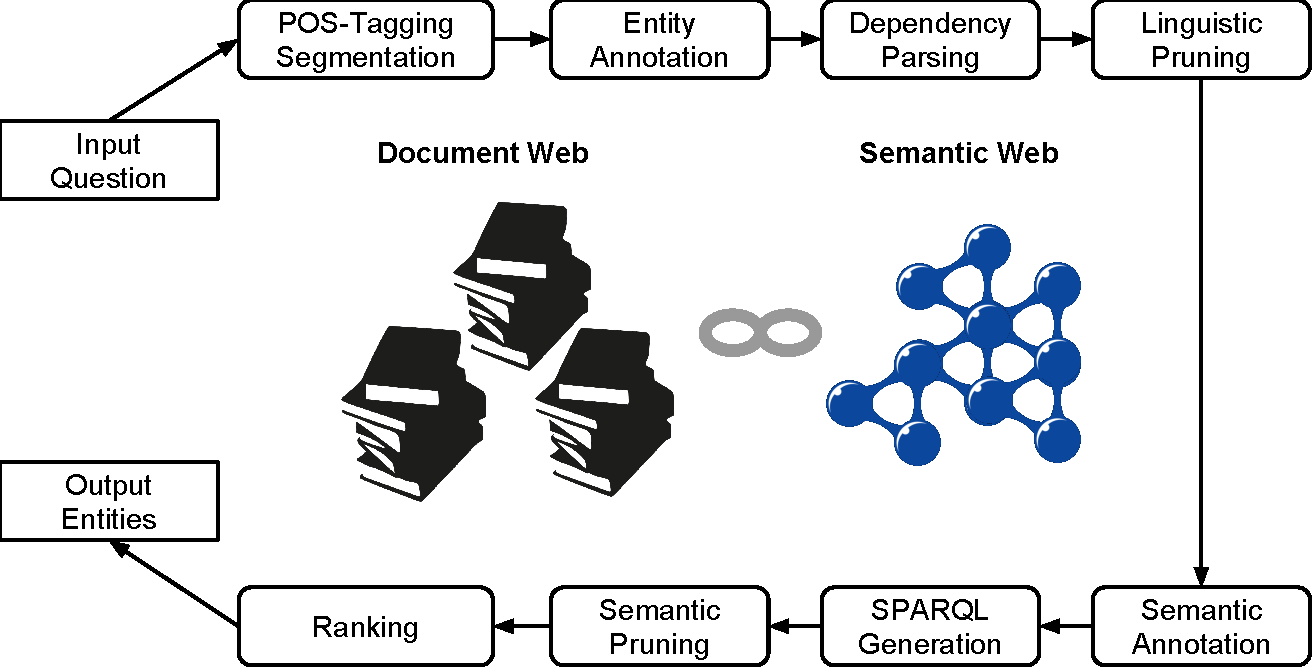
\includegraphics[width=0.8\linewidth]{part_03/ESWC_HAWK/HAWK_architecture}
\caption{Architectural overview of HAWK.}
\label{chahawk:fig:architecture}
\end{figure}


\subsection{POS-Tagging, Segmentation}
%\todo[inline]{re is no tokenisation/segmentation component in the pipeline?}
A large number of frameworks have been developed for these purposes over the last years. 
We rely on \emph{clearNLP}~\cite{choi2011getting} which is based on transition-based dependency parsing and sophisticated segmentation algorithm.
Regarding our running example the following POS-tags are generated:
\texttt{Which(WDT) recipients(NNS) of(IN) the(DT) Victoria(NNP) Cross(NNP) died(VBN) in(IN) the(DT) Battle(NNP) of(IN) Arnhem(NNP)?(PUNCT)}

\subsection{Entity Annotation}
HAWK identifies named entities and tries to link them to semantic entities from the underlying knowledge base, in our case DBpedia 3.9, via well-established entity annotation tools, also called entity tagging tools:
\begin{itemize}
\item \textbf{Wikipedia Miner}~\cite{milne2008learning} is based on different facts like prior probabilities, context relatedness and quality, which are then combined and tuned using a classifier.
\item \textbf{DBpedia Spotlight}~\cite{spotlight} %, one of the first semantic entity annotation approaches, 
was published in 2011. 
This tool combines named entity recognition and disambiguation based on DBpedia.
\item \textbf{TagMe 2}~\cite{TagMe2} is based on a directory of links, pages and an inlink graph from Wikipedia.
The approach recognizes entities by matching terms with Wikipedia link texts and disambiguates the match using the in-link graph and the page dataset.
%Afterwards, TagMe 2 prunes identified named entities which are considered as non-coherent to the rest of the named entities in the input text.  
\item \textbf{FOX}~\cite{FOX} has been introduced 2014 as an ensemble learning-based approach combining several state-of-the-art named entity recognition approaches. 
The FOX framework outperforms the current state of the art entity recognizers and relies on the entity linking tool AGDISTIS~\cite{agdistis_iswc}.
\end{itemize}
Additionally, we implemented two artificial spotters for evaluation:
\begin{itemize}
\item \textbf{Union} is a spotter that combines the result sets of the above introduced spotters and returns thus a superset of all spotters.
\item \textbf{Optimal} will spot all entities from the gold standard to be able to ignore spotting influences in the following steps of the pipeline.
\end{itemize}

For our running example, an optimal spotter identifies \texttt{Victoria\_Cross} and \texttt{Battle\_of\_Arnhem} as resources form DBpedia.
HAWK annotates the POS-tag \texttt{ADD} to it. % for our running example from above.
The influence of the entity annotation module is evaluated in Section~\ref{chahawk:sec:evaluation}.

\subsection{Dependency Parsing}
HAWK performs noun phrase detection for semantically meaningful word groups not yet recognized by the entity annotation system also known as chunking.
This detection reuses the above mentioned POS-tagger. % based on a-priori part-of-speech (POS) tagging~\cite{choi2011getting}.
Input tokens will be combined following manually-crafted linguistic heuristics derived from the benchmark questions, and their POS-tag is changed to \texttt{CNN}.
Thus, the input is a natural language question (list of keywords) and the output is a list of chunks, see Algorithm~1.
HAWK's modular structure allows for an easy exchange of the POS-tagger or dependency parser.

\begin{algorithm}[tb!]
\SetAlgoLined
\KwData{Tokenized question ($list$) with Part-of-Speech-tags (POS-tags)}
	subsequence = ()\;
	\For{$t \in [0,|list|]$ }{
			token = list.get($t$)\;
			%// look for start "RB|JJ|NN(.)*"
			\eIf{$subsequence = \emptyset$}{
			    \lIf{$pos(t) \in (\mathrm{CD|JJ|NN(.)^*|RB(.)^*})$} {
				subsequence.add(token)
				}
			}
			%// split "of the" or "of all" via pos\_i=IN and pos\_i+1=DT
			{
    			\uIf{$t + 1 < |list| \wedge pos(t) \in (\mathrm{IN}) \wedge pos(t+1) \in (\mathrm{(W)?DT})$} {
    				\lIf{$subsequence.size() >= 2$} {
    					combine(subsequence)
    				}
    		        subsequence = ()\;
    			}
    		%	// do not combine NNS and NNPS but combine "stage name", "British Prime minister"
    			\uElseIf{$pos(t - 1) \in (\mathrm{NNS}) \wedge pos(t) \in (\mathrm{NNP(S)?})$} {
    			    \lIf{$subsequence.size() > 2$} {
    					combine(subsequence)
    				}
    		        subsequence = ()\;
    			}
    		%	// finish via VB* or IN -> null or IN -> DT or WDT (now a that or which follows)
    			\uElseIf{$!pos(t - 1) \in (\mathrm{JJ|HYPH}) \wedge (pos(t) \in (\mathrm{VB|WDT|IN})))$} {
    		%		// more than one token, so summarizing makes sense
    			    \lIf{$subsequence.size() > 1$} {
    					combine(subsequence)
    				}
    		        subsequence = ()\;
    			}
    		    \uElseIf{$pos(t) \in (\mathrm{NN(.)^*|RB|CD|CC|JJ|DT|IN|PRP|HYPH|VBN})$} {
    				subsequence.add(token)
    			}
    			\uElse{
    		        subsequence = ()\;
    			}
    		}
        }
\caption{Algorithm for combining noun phrases.}
\label{listing:nouncombiner}
\end{algorithm}



Subsequently, in order to capture linguistic and semantic relations, HAWK parses the query using dependency parsing and semantic role labeling~\cite{choi2011getting}.
The dependency parser is given the chunked question. 
The generated pre\-dicate-argument tree is directed, acyclic, and all its nodes contain their POS-tags as well as their labels, see Figure~\ref{chahawk:fig:dependency_tree}.


\subsection{Linguistic Pruning}

The natural language input can contain tokens that are meaningless for retrieving the target information or even introduce noise in the process.
HAWK therefore prunes nodes from the predicate-argument tree based on their POS-tags, e.g., deleting all \texttt{DET} nodes, interrogative phrases such as \texttt{Give me} or \texttt{List}, and auxiliary tokens such as \texttt{did}.
Algorithm~2 details the algorithm for removing nodes.
Figure~\ref{chahawk:fig:prunedtree} depicts the predicate-argument tree obtained for our running example after pruning.% of unnecessary nodes.

\begin{algorithm}[tb!]
\SetAlgoLined
\KwData{Dependency-argument tree with Part-of-Speech-tags}
Queue queue = [tree.getRoot()]\;
\While{$queue != \emptyset$} {
	node = queue.poll()\;
    \If{$pos(node) \in (\mathrm{WDT|POS|WP\$|PRP\$|RB|PRP|DT|IN|PDT})$} {
	tree.remove(node)\;
}
	queue.add(node.getChildren())\;
}
\If{$root.label == ("Give")$} {
	\For{$childNode \in root.getChildren()$} {
		\lIf{$childNode == "me"$} {
			tree.remove(childNode)
		}
	}
}
\lIf{root.label $\in\{ "List", "Give"\}$}{
	tree.remove(root)
}
\caption{Algorithm for pruning noisy nodes}
\label{listing:lingpruning}

\end{algorithm}


\begin{minipage}{0.57\textwidth} 
\centering

\includegraphics[width=\linewidth]{part_03/ESWC_HAWK/hawk_tree_full}
\captionof{figure}{Predicate-argument tree for the example question `Which recipients of the Victoria Cross died in the Battle of Arnhem?'}
\label{chahawk:fig:dependency_tree}
\end{minipage}
\hfill
\begin{minipage}{0.36\textwidth}
\centering

\includegraphics[width=\linewidth]{part_03/ESWC_HAWK/hawk_tree_pruned}
\captionof{figure}{Tree after pruning. Argument edges are ordered from left to right.}
\label{chahawk:fig:prunedtree}
\end{minipage}

\subsection{Semantic Annotation}
After linguistic pruning, HAWK annotates each node in the tree with possible concepts from the knowledge base and its underlying ontology.
To this end, our framework uses information about possible verbalizations of ontology concepts, based on both \texttt{rdfs:label} information from the ontology itself and (if available) verbalization information contained in lexica.
%lexiconexisting manually crafted English lexicon\footnote{\url{https://github.com/cunger/lemon.dbpedia}} for DBpedia. 
% we generated triples of the form $\langle$\emph{reference},\,\texttt{rdfs:label},\,\texttt{"}\emph{form}\texttt{"}$\rangle$, that link an ontology element (\emph{reference}) to its written representation (\emph{form}) in the lexicon. 
In general, such lexica offer a range of lexical variants beyond the labels present in DBpedia. For example, for the property \texttt{spouse}, the DBpedia English lexicon\footnote{\url{https://github.com/cunger/lemon.dbpedia}} provides the noun entries `wife' and `husband' as well as the verb entry `to marry'.
%, 
%resulting in the following triples:

%\begin{itemize}
%\item \texttt{http://dbpedia.org/ontology/spouse rdfs:label "wife" .}
%\item \texttt{http://dbpedia.org/ontology/spouse rdfs:label "husband" .}
%\item \texttt{http://dbpedia.org/ontology/spouse rdfs:label "marry" .}
%\end{itemize}

HAWK now tries to match each node label to a class or property from the DBpedia ontology using fuzzy string matching.
%with an edit distance of 1 as provided by the Lucene framework\footnote{\url{http://lucene.apache.org/}}.
Moreover, HAWK follows intuitions used in~\cite{tbsl} to lower the number of annotations avoiding additional computational effort. 
In particular, we consider the POS-tag of nodes to determine the type of the target reference:
\begin{itemize}
\item nouns correspond to object type properties and classes
\item verbs correspond to object type properties
\item question words (e.g., \texttt{who} or \texttt{where}) correspond to classes (e.g., \texttt{Person} or \texttt{Place})
\end{itemize}

Afterwards, HAWK ranks properties according to their prominence score in the knowledge base and returns only the top n properties.
If the search does not retrieve any annotations, we additionally ask the lemmata of the node label and repeat the above described process to increase recall.

Considering our running example,the nodes \texttt{died (VB)} will be annotated with \texttt{dbo:deathplace} and \texttt{dbo:deathdate} and the node \texttt{recipients (NNS)} with \texttt{dbo:award}.
After this step, either a node is annotated with a reference from the knowledge base % it is a disambiguated resource 
or it will be lead to a full-text lookup to be resolved to a knowledge base resource as explained in the following section.

%\begin{table}[htb]
%\caption{Annotations of nodes from running example.}
%\centering
%    \begin{tabular}{ll}
%        \toprule
%             & \textbf{Annotation}\\
%        \midrule
%            died& \texttt{dbo:deathplace}, \texttt{dbo:deathdate} \\
%            recipients & \texttt{dbo:award} \\
%        \bottomrule
%    \end{tabular}
%\label{tab:annotations}
%\end{table}

\subsection{Generating SPARQL Queries}
\label{chahawk:sec:full-text}

The core of HAWK is the generation of SPARQL queries from annotated and pruned predicate-argument trees.
%\todo[inline]{The indexed properties used for  text searches will be described in Section 2.6. }
It uses an Apache Jena FUSEKI\footnote{\url{http://jena.apache.org/documentation/serving_data/}} server, which implements the full-text search predicate \texttt{text:query} on a-priori defined literals over configured predicates. % using the Lucene search query syntax. 
Especially, the following predicates were indexed as they yield a high information content with respect to DBpedia 3.9:
\begin{itemize}
 \item \texttt{dbpedia:abstract} for general interest information about a resource not modelled appropriately in the knowledge base
 \item \texttt{rdfs:label} to match resources not found by the entity annotation system%, e.g., \url{http://dbpedia.org/resource/The\_Crown}
 \item \texttt{dbpedia:redirect} to identify common synonyms, e.g., `first man in space' pointing to \url{http://dbpedia.org/resource/Yuri_Gagarin}
 \item \texttt{dc:subject} for linking top-level categories like `assassin' to resources like \url{http://dbpedia.org/resource/James_Earl_Ray}
\end{itemize}
Currently, HAWK resolves full-text information either by using exact matches of node labels or fuzzy matches on each non-stopword token of a label; Table~\ref{tab:exact_fuzzy} depicts the two possibilities for the running example.

\begin{table}[htb!]
\centering
\caption{Examples for full-text query types.}
\begin{tabular}{l@{\quad}l@{\quad}l}
\toprule
\textbf{Query Type} & \textbf{Query Syntax} & \textbf{Node label}\\
\midrule
Exact & \texttt{?var text:query ('Battle of Arnhem')}  & Battle of Arnhem\\
Fuzzy & \texttt{?var text:query ('Battle\textasciitilde1 AND Arnhem\textasciitilde 1')} & Battle of Arnhem\\
\bottomrule
\end{tabular}
\label{tab:exact_fuzzy}
\end{table}
To capture the full semantics of an input question, HAWK traverses the predicated-argument tree in a pre-order walk to reflect the empirical observation that i) related information are situated close to each other in the tree and ii) information are more restrictive from left to right.
This breadth-first search visits each node and generates several \emph{possible triple patterns} based on the number of annotations and the POS-tag itself. 
That is, for each node a set of SPARQL query patterns is generated following the rules depicted in Table~\ref{tab:triple_patterns} w.r.t. ontology type information, e.g., a variable bound to the class \texttt{Place} will not have an outgoing predicate \texttt{birthPlace}.

Using this approach allows HAWK to be independent of SPARQL templates %, such as used by TBSL~\cite{tbsl}, 
and to work on natural language input of any length and complexity.
Each pattern contains at least one variable from a pre-defined set of variables, i.e., \texttt{?proj} for the resource projection variable, \texttt{?const} for resources covering constraints related to the projection variable as well as a variety of variables for predicates to inspect the surrounding of elements in the knowledge base graph. 
Table~\ref{tab:triple_patterns_example} shows generated triple patterns for parts of the example query.
\begin{table}[htb!]
\centering
\caption{Generated triple patterns for running example.}
\begin{tabular}{l@{\quad}l}
\toprule
\textbf{Node Type} & \textbf{Query Fragment} \\
\midrule
\multirow{2}{*}{CNN} & \texttt{?proj text:query ('Battle of Arnhem')} \\
& \texttt{?const text:query ('Battle of Arnhem')} \\
%& \texttt{?proj text:query ('Battle~1 AND Arnhem~1')} \\
%& \texttt{?const text:query ('Battle~1 AND Arnhem~1')}\\
\midrule
\multirow{2}{*}{Verb} & \texttt{?proj dbo:deathPlace ?const} \\
 & \texttt{?const dbo:deathPlace ?proj} \\
\bottomrule
\end{tabular}

\label{tab:triple_patterns_example}
\end{table}

\begin{table}[htb!]
\centering
\caption{Triple patterns for generating SPARQL queries while traversal.}
\begin{tabular}{ll}
\toprule
\textbf{Node POS-tag and non-empty annotations} & \textbf{Query Fragment} \\
\midrule
VB(.)* & \texttt{?proj Annotation ?const.} \\
VB(.)* & \texttt{?const Annotation ?proj.} \\
VB(.)* & \texttt{?const ?proot ?proj.} \\
NN(.)*$|$WRB & \texttt{?proj  Annotation ?const.} \\
NN(.)*$|$WRB & \texttt{?const Annotation ?proj.} \\
NN(.)*$|$WRB & \texttt{?proj a Annotation.} \\
NN(.)*$|$WRB & \texttt{?const a Annotation.} \\
NN(.)*$|$WRB & \texttt{?const text:query (node label)} \\
WP& \texttt{?const a Annotation.} \\
WP& \texttt{?proj a Annotation.} \\
%WP$|$NN(.)*$|$WRB& ignore \\
in all cases & add empty triple pattern\\
\midrule
\textbf{Node POS-tag and empty annotations} & \textbf{Query Fragment} \\
\midrule
CNN$|$NNP(.)*$|$JJ$|$CD&  \texttt{?proj text:query (node label)} \\
CNN$|$NNP(.)*$|$JJ$|$CD&\texttt{?const text:query (node label)} \\
VB(.)*& \texttt{?proj text:query (node label)} \\
VB(.)*&\texttt{?const text:query (node label)} \\
ADD& \texttt{?proj ?pbridge nodeURI.} \\
ADD& \texttt{FILTER (?proj IN (nodeURI))} \\
ADD&  \texttt{?proj text:query (node label)} \\
ADD& \texttt{?const text:query (node label)} \\
NN$|$NNS& \texttt{?proj text:query (node label)} \\
NN$|$NNS& \texttt{?const text:query (node label)} \\
%NN(.)*$|$WP$|$ADD$|$VB(.)*$|$CombinedNN$|$JJ$|$CD& ignore node \\
in all cases & add empty triple pattern \\
\bottomrule
\end{tabular}

\label{tab:triple_patterns}
\end{table}

During this process, each iteration of the traversal appends the generated patterns to each of the already existing SPARQL queries. 
This combinatorial effort results in covering every possible SPARQL graph pattern given the predicate-argument tree.



\subsection{Semantic Pruning of SPARQL Queries}

Producing the n-fold-cross-product of possible pattern combinations generates a huge number of SPARQL queries, most of which are semantically senseless,e.g., a city that has a birth date. 
To effectively handle this large set of queries and reduce the computational effort, HAWK implements various methods for pruning:
\begin{itemize}
\item \textbf{\#textfilter: } HAWK can safely assume that SPARQL queries containing full-text lookups over more than one variable or containing more than two node labels do not yield semantically senseful information and thus discards such queries. 
\item \textbf{\#unbound triple pattern}: SPARQL queries containing more than one triple pattern of the form \texttt{?varx ?vary ?varz} or one such triple pattern and only text searches, lead to a traversal of large parts of the knowledge base graph and high computational effort.
\item \textbf{Unconnected query graph: } SPARQL query graphs which are not connected from cartesian products are pruned for the sake of runtime and their lack of semantics.
\item \textbf{Cyclic triple: } Queries containing edges of the form \texttt{?s <http://xyz>  ?o. ?o <http://xyz> ?s} or \texttt{?s <http://xyz>  ?o. ?s <http://abc> ?o} are also removed. 
\item \textbf{Missing projection variable: } The before mentioned traversal and SPARQL generation process can produce SPARQL queries without triple patterns containing the projection variable. These queries are also removed from the set of queries.
\item \textbf{Disjointness: }
Also SPARQL queries with triple patterns violating disjointness statements are discarded:
\begin{itemize}
\item \texttt{?s a  cls . ?s p ?o .} if \texttt{cls} and domain of \texttt{p} are disjoint
\item \texttt{?o a  cls . ?s p ?o .} if \texttt{cls} and range of \texttt{p} are disjoint
\item \texttt{?s p1  ?o1 . ?s p2 ?o2 .} if domain of \texttt{p1} and \texttt{p2} are disjoint
\item \texttt{?s1 p1  ?o . ?s2 p2 ?o .} if range of \texttt{p1} and \texttt{p2} are disjoint
\item \texttt{?s p1  ?o . ?s p2 ?o .} if \texttt{p1} and \texttt{p2} are disjoint
\end{itemize}
Due to lack of explicit disjointness statements in many knowledge bases, we (heuristically) assume that classes and properties that are not related via subsumption hierarchy are disjoint.
%\item \textbf{Entity type mismatch: }\todo[inline]{Eigentlich sollte das ja schon beim entity lookup passieren, d.h. es macht Sinn für predicate auch nur in der Menge der properties zu suchen, dasselbe gilt für Klassen. eher ungünstig das hier überhaupt zu erwähnen, lässt unseren lookup nicht sehr schlau aussehen, und ist auch trivial.}
\end{itemize}

Although semantic pruning drastically reduces the amount of queries, it often does not result in only one query. HAWK thus requires a final ranking step before sending the SPARQL query to the target triple store.

\subsection{Ranking}
%\todo[inline]{motivate features more}
HAWK ranks queries using supervised training based on the gold standard answer set from the QALD-4 benchmark.
In the \emph{training phase}, all generated queries are run against the underlying SPARQL endpoint. 
Comparing the results to the gold standard answer set, HAWK stores all queries resulting with the same high F-measure.
Afterwards the stored queries are used to calculate an average feature vector comprising simple features mimicking a centroid-based cosine ranking.
HAWK's ranking calculation comprises the following components:
\begin{itemize}
\item \textbf{NR\_OF\_TERMS} calculates the number of nodes used to form the full-text query part as described in Section~\ref{chahawk:sec:full-text}.
\item \textbf{NR\_OF\_CONSTRAINTS} counts the amount of triple patterns per SPARQL query.
\item \textbf{NR\_OF\_TYPES} sums the amount of patterns of the form \texttt{?var rdf:type cls}.
\item \textbf{PREDICATES} generates a vector containing an entry for each predicate used in the SPARQL query.
%\item \textbf{2path motifs containing a variable with a text:filter}
%\todo[inline]{Paste picture of motifs here}
\end{itemize}

While running the \emph{test phase} of HAWK, the cosine similarity between each SPARQL query using the above mentioned features and the average feature vector of training queries is calculated.
Moreover, HAWK determines the target cardinality $x$, i.e., \texttt{LIMIT x}, of each query using the indicated cardinality of the first seen POS-tag of the input query, e.g., the POS-tag \texttt{NNS} demands the plural while \texttt{NN} demands the singular case and thus leads to different \texttt{x}.
The performance of this ranking approach is evaluated in Section~\ref{chahawk:sec:evaluation}.
%\todo[inline]{Show two queries, their vectors and their score.}

%\subsection{Demo}
%\begin{itemize}
%\item test queries
%\item verbalisation
%\item feedback loop?
%\end{itemize}


\section{Evaluation}
\label{chahawk:sec:evaluation}

\subsection{Benchmark}

We evaluate HAWK against the QALD~\cite{qald4} benchmark.
%The available benchmarks target diverse domains such as medicine, music or general knowledge. 
QALD has been used widely to evaluate question answering systems, e.g., TBSL, SINA, FREyA or QAKiS, which are presented in Section~\ref{chahawk:sec:relatedwork}.
In the recent fourth installment of QALD, hybrid questions on structured and unstructured data became a part of the benchmark.
To evaluate HAWK, we focus on this hybrid training dataset comprising 25 questions, 17 out of which are entity searches using only DBpedia type information, no aggregation process and require only \texttt{SELECT}-queries. 
The available test dataset comprises only 10 question with 6 entity searches and linguistic structures that are completely different from the training dataset.
Before evaluation, we had to curate the benchmark datasets regarding, among others, incorrect grammar, typological errors, duplicate resources in the answer set.
The cleaned datasets can be found in our source code repository.\footnote{\url{https://github.com/AKSW/hawk/tree/master/resources}}
Without this correction HAWK's f-measure shrinks to nearly zero for questions containing failures.
To the best of our knowledge there is no other published approach on hybrid question answering.
%Table~\ref{tab:datasets} details properties of the used dataset.
 
\subsection{Influence of the Entity Annotation System}
First, we evaluated the influence of the applied entity annotation systems to the overall ability to produce correct answers.
Thus, HAWK has been run using DBpedia Spotlight, TagMe, Fox and Wikipedia Miner. 
Additionally, an optimal entity annotator derived from the gold standard as well as an union of all entity annotation results was analysed. %while assuming with an perfect ranking systems. %, see Figure~\ref{chahawk:fig:spiderOfEntityAnnotators}.

%\begin{figure}
%\centering
%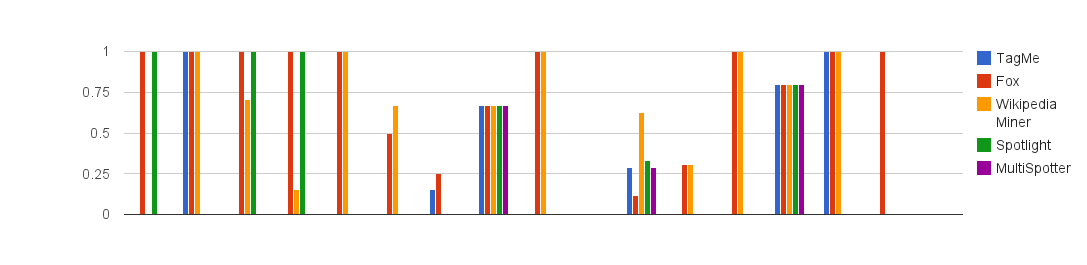
\includegraphics[width=\linewidth]{bars}
%\caption{Entity annotations systems performance with optimal ranking}
%\label{chahawk:fig:spiderOfEntityAnnotators}
%\end{figure}
Our results suggest that HAWK is able to retrieve correct answers with an F-measure of 0.68 using FOX as entity annotation system and assuming an optimal ranking.
Furthermore, the optimal ranker is only able to achieve an F-measure of 0.58 since HAWK can cope better with missing annotation results and is tuned towards retrieving full-text information.
Against intuition, the Union annotator is the worst annotation system. 
Merging all annotation results in queries consisting solely of semantic resources eliminating the possibility to match ontology properties and classes to important parts of the query, e.g., matching the word \texttt{author} to resource rather than to a property prevents HAWK from generating the correct SPARQL query.
Thus, the Union annotator achieves only an F-measure of 0.10.\footnote{Details on this evaluation can be found in the supplement on our project homepage.}


\subsection{Influence of the Ranking Method}
Next, evaluating the effectiveness of the feature-based ranking has to include an in-depth analysis of the contribution of each feature to the overall result.
Thus, we calculated the power set of the set of features and evaluated each feature group using the F-measure reached by the top n queries. 
Figures~\ref{chahawk:fig:ranking_1} and ~\ref{chahawk:fig:ranking_2} show the F-measure@N for all query result sets of size $N$ from all 17 questions. 
%\todo[inline]{What exactly is shown in Figure 4 - i.e. there are F1/Precision/Recall scores for each of the 17 questions the system could answer, but how is the score calculated? I.e. either the systems get the right answer or not? Or is this based on top-N answers? Or based on how many correct answers from all the candidate queries?}
%\begin{minipage}{0.49\textwidth} 
%\centering
\begin{figure}[htb!]
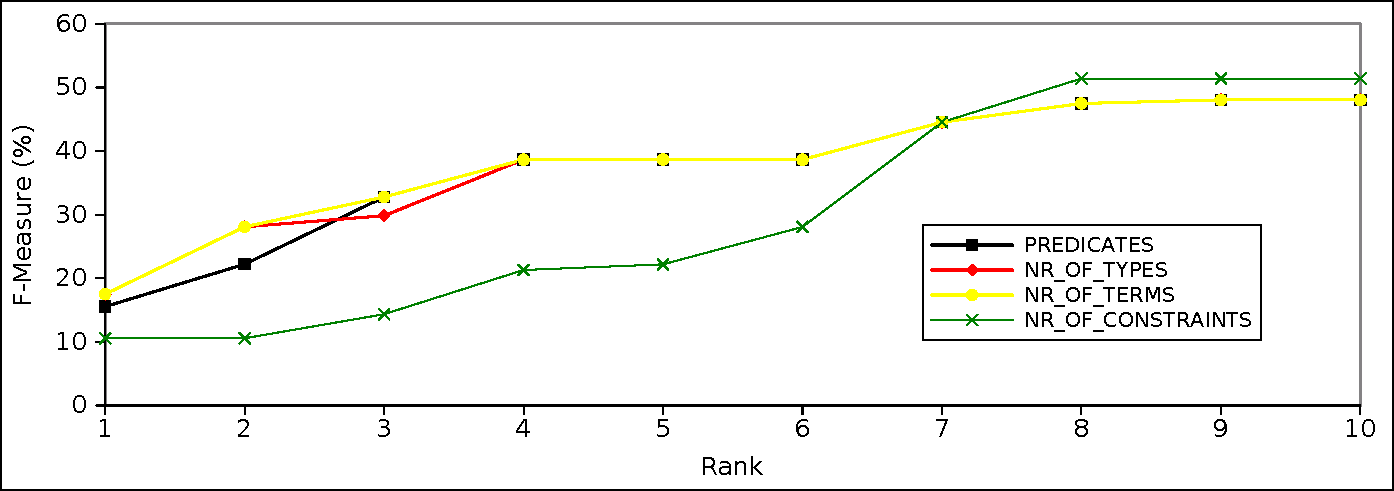
\includegraphics[width=\linewidth]{part_03/ESWC_HAWK/onefeature}
%\captionof{figure}{F-measures on training dataset using $N=[1,\ldots,10]$ and one feature.}
\caption{F-measures on training dataset using $N=[1,\ldots,10]$ and one feature.}
\label{chahawk:fig:ranking_1}
\end{figure}
%\end{minipage}
%\hfill
%\begin{minipage}{0.49\textwidth}
%\centering
\begin{figure}[htb!]
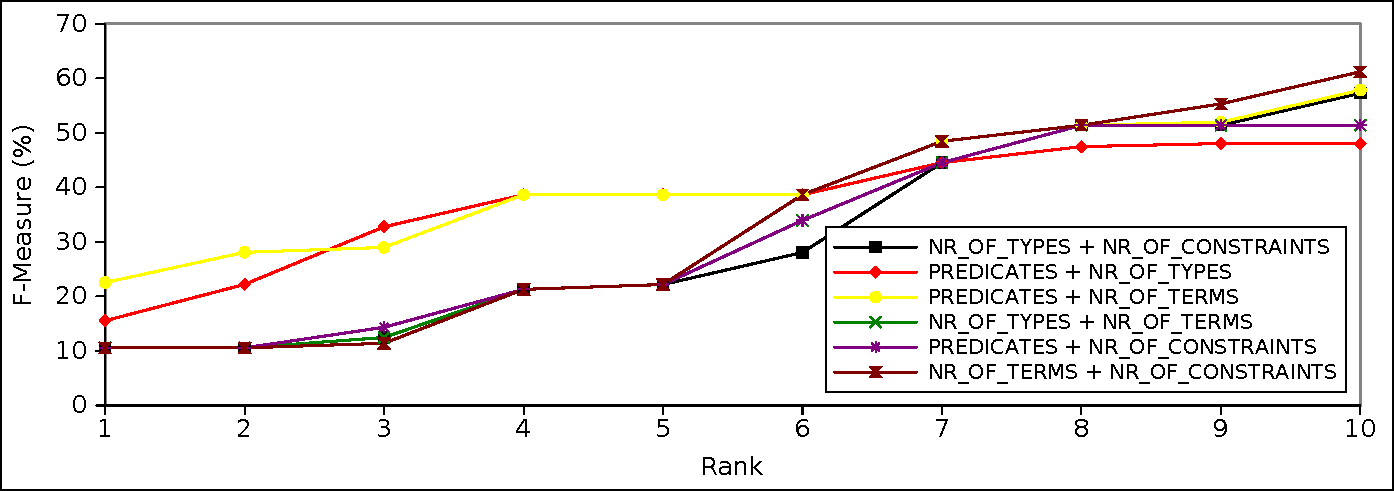
\includegraphics[width=\linewidth]{part_03/ESWC_HAWK/twofeature}
%\captionof{figure}{F-measures on training dataset using $N=[1,\ldots,10]$ and two features.}
\caption{F-measures on training dataset using $N=[1,\ldots,10]$ and two features.}
\label{chahawk:fig:ranking_2}
\end{figure}
%\end{minipage}

%\begin{minipage}{0.49\textwidth} 
%\centering
%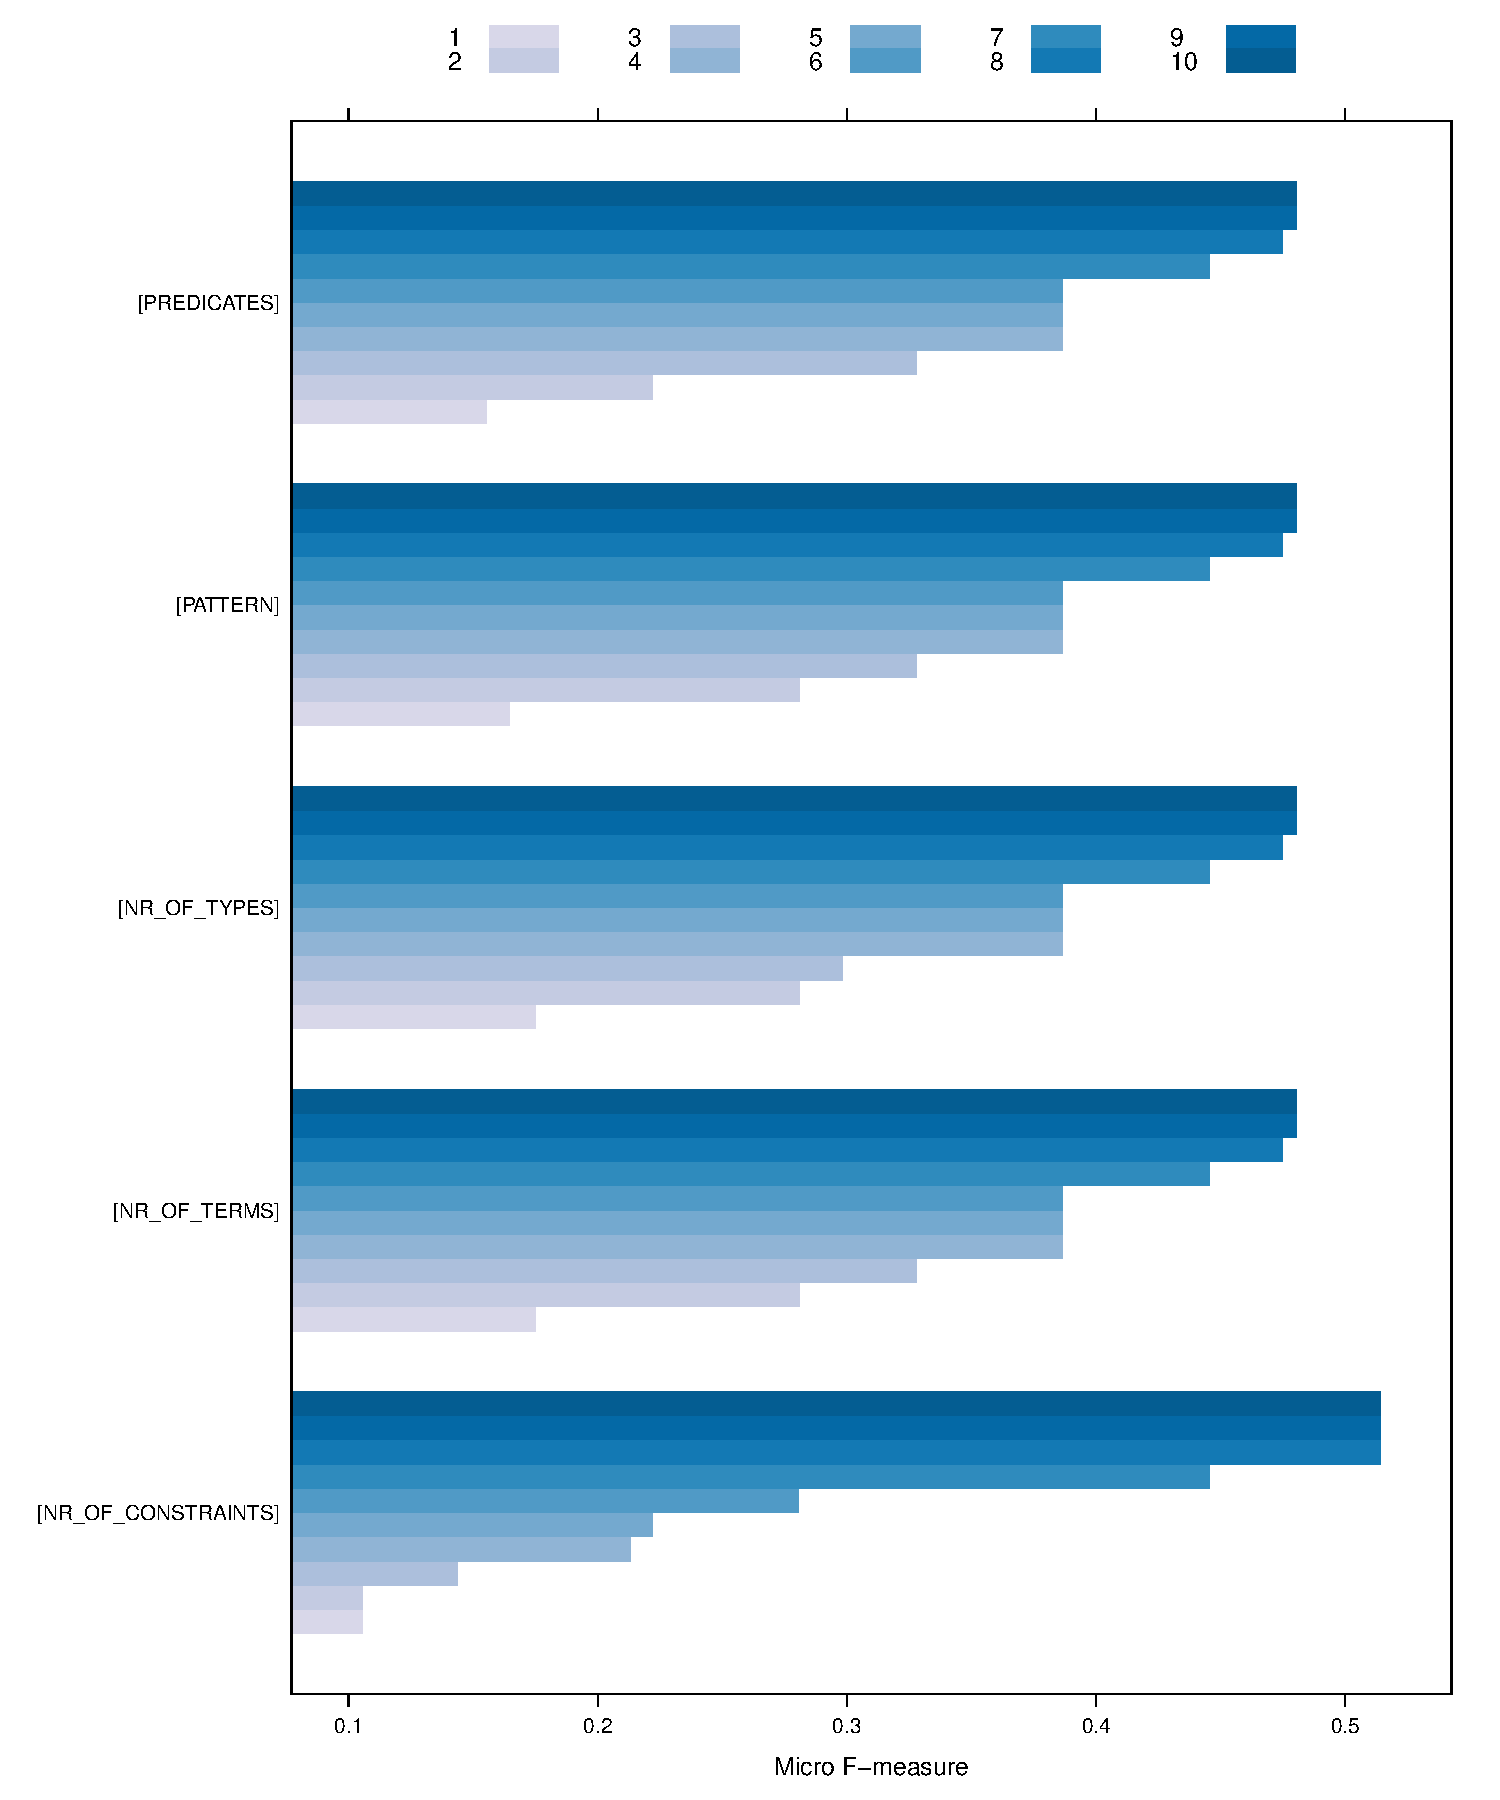
\includegraphics[width=\linewidth]{ranking_1}
%\captionof{figure}{F-measures on training dataset using $N=[1,\ldots,10]$ and one feature.}
%\label{chahawk:fig:ranking_1}
%\end{minipage}
%\hfill
%\begin{minipage}{0.49\textwidth}
%\centering
%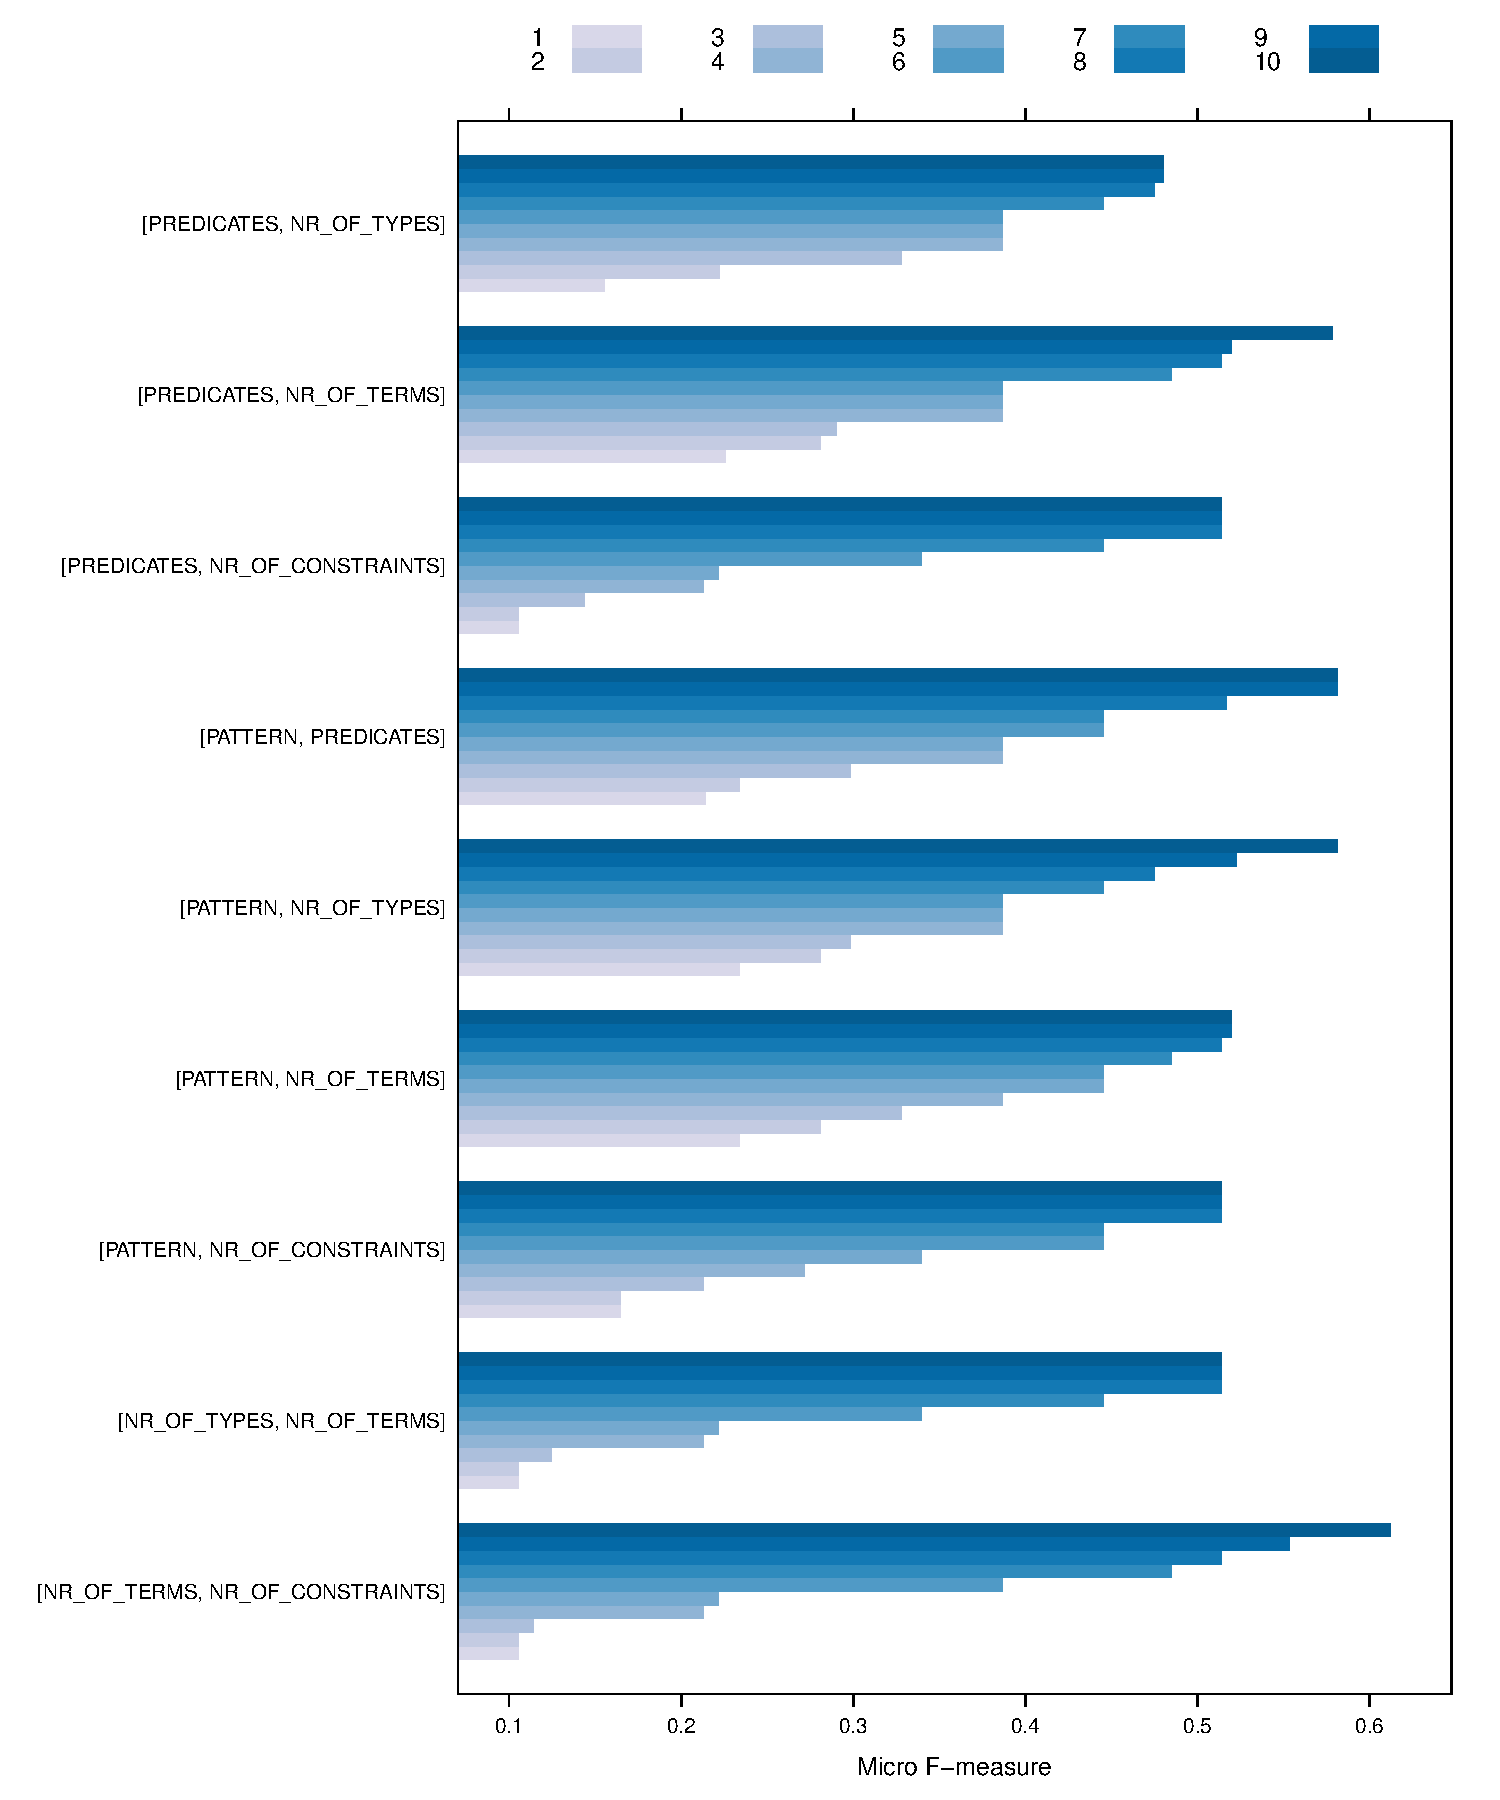
\includegraphics[width=\linewidth]{ranking_2}
%\captionof{figure}{F-measures on training dataset using $N=[1,\ldots,10]$ and two features.}
%\label{chahawk:fig:ranking_2}
%\end{minipage}

%\begin{minipage}{0.49\textwidth} 
%\centering
%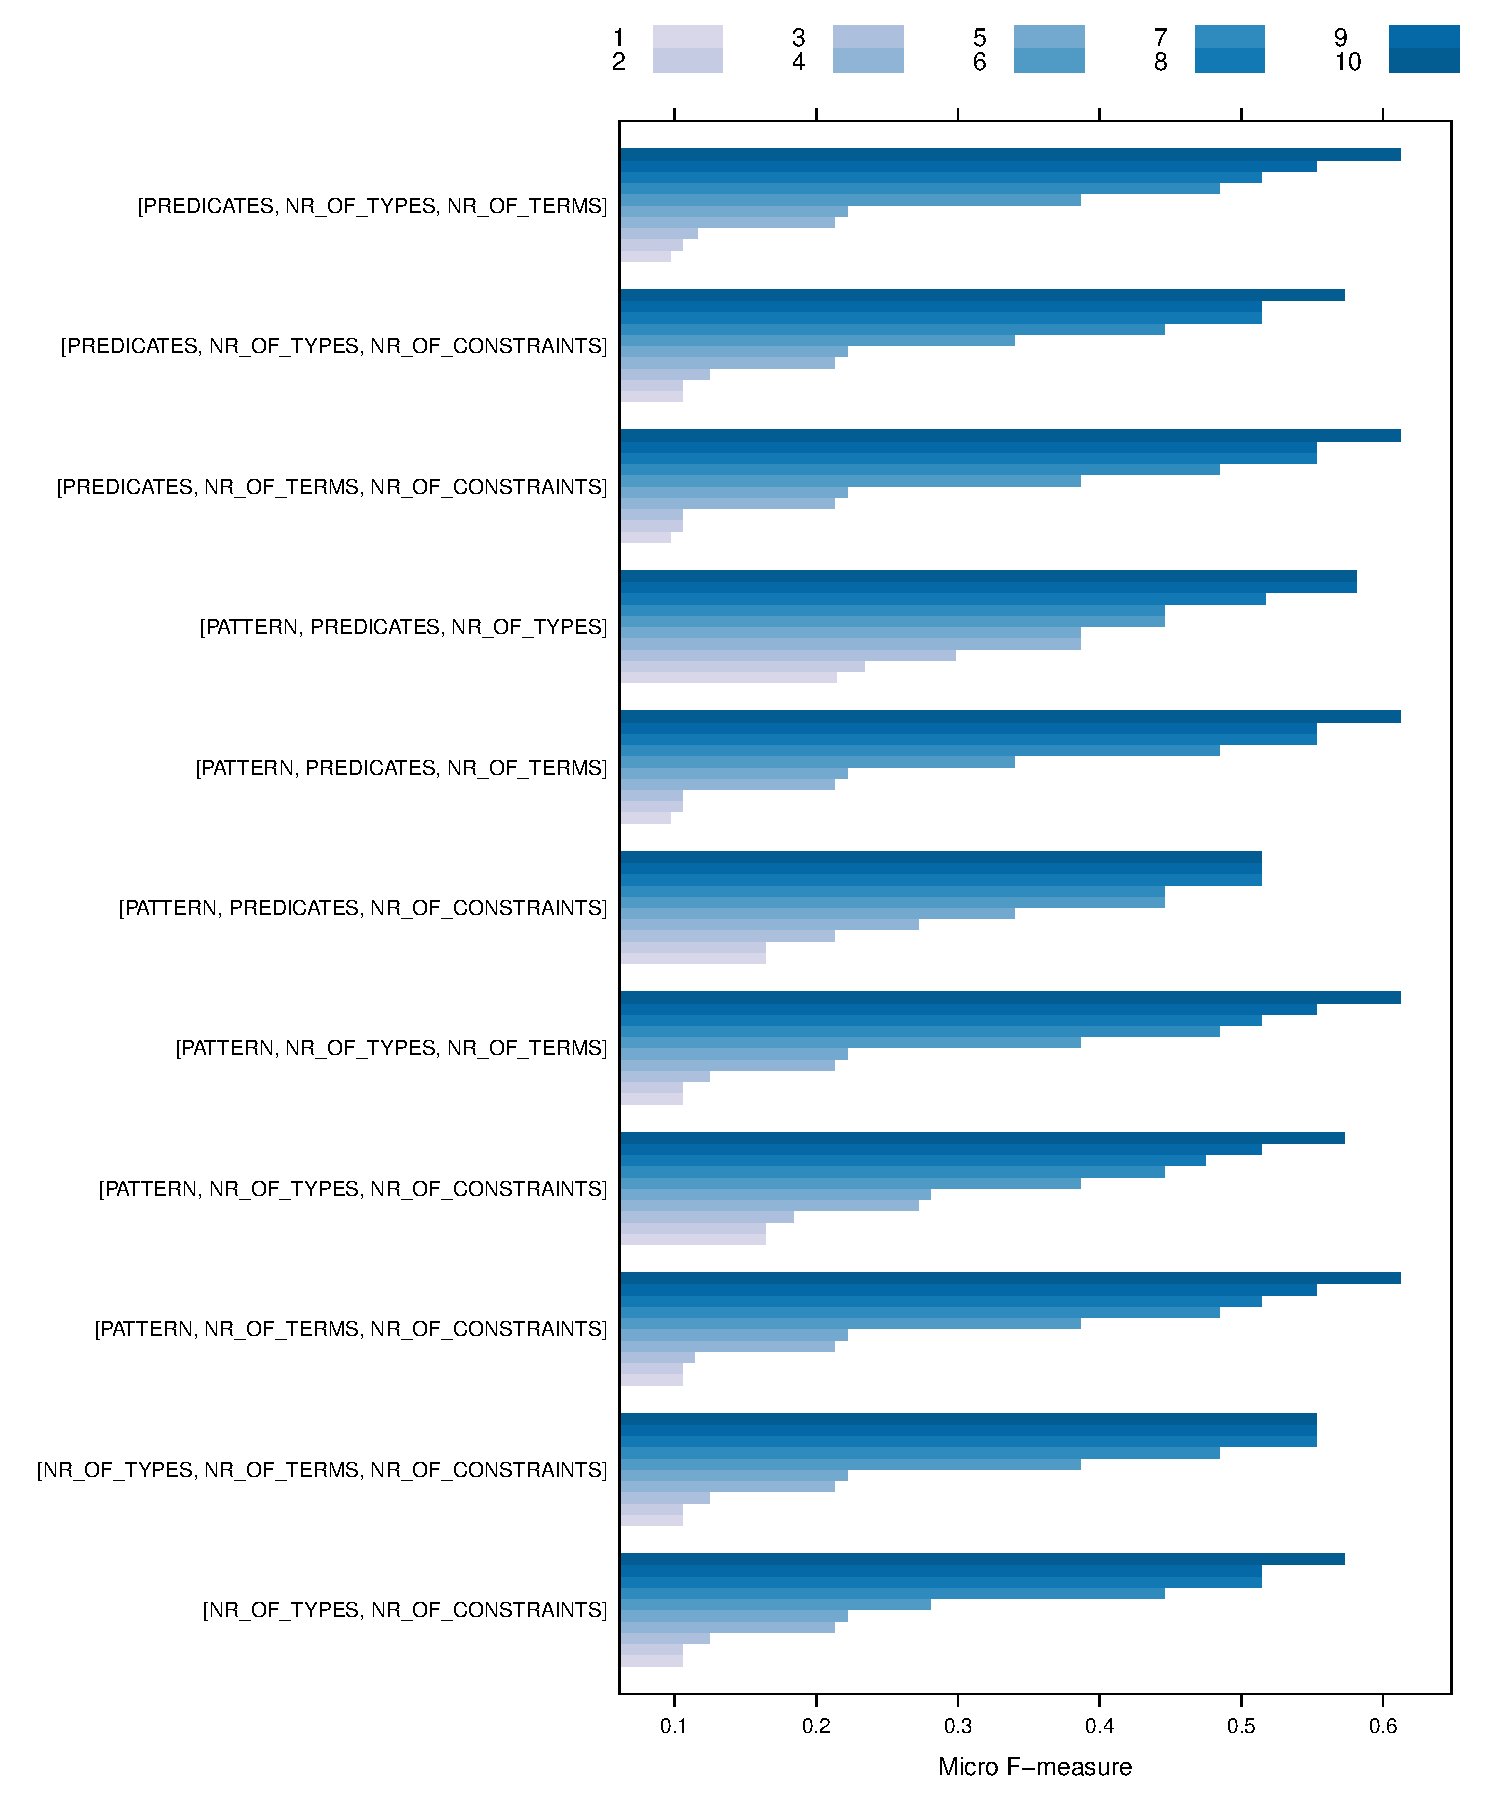
\includegraphics[width=\linewidth]{ranking_3}
%\captionof{figure}{F-measures on training dataset using $N=[1,\ldots,10]$ and three features.}
%\label{chahawk:fig:ranking_3}
%\end{minipage}
%\hfill
%\begin{minipage}{0.49\textwidth}
%\centering
%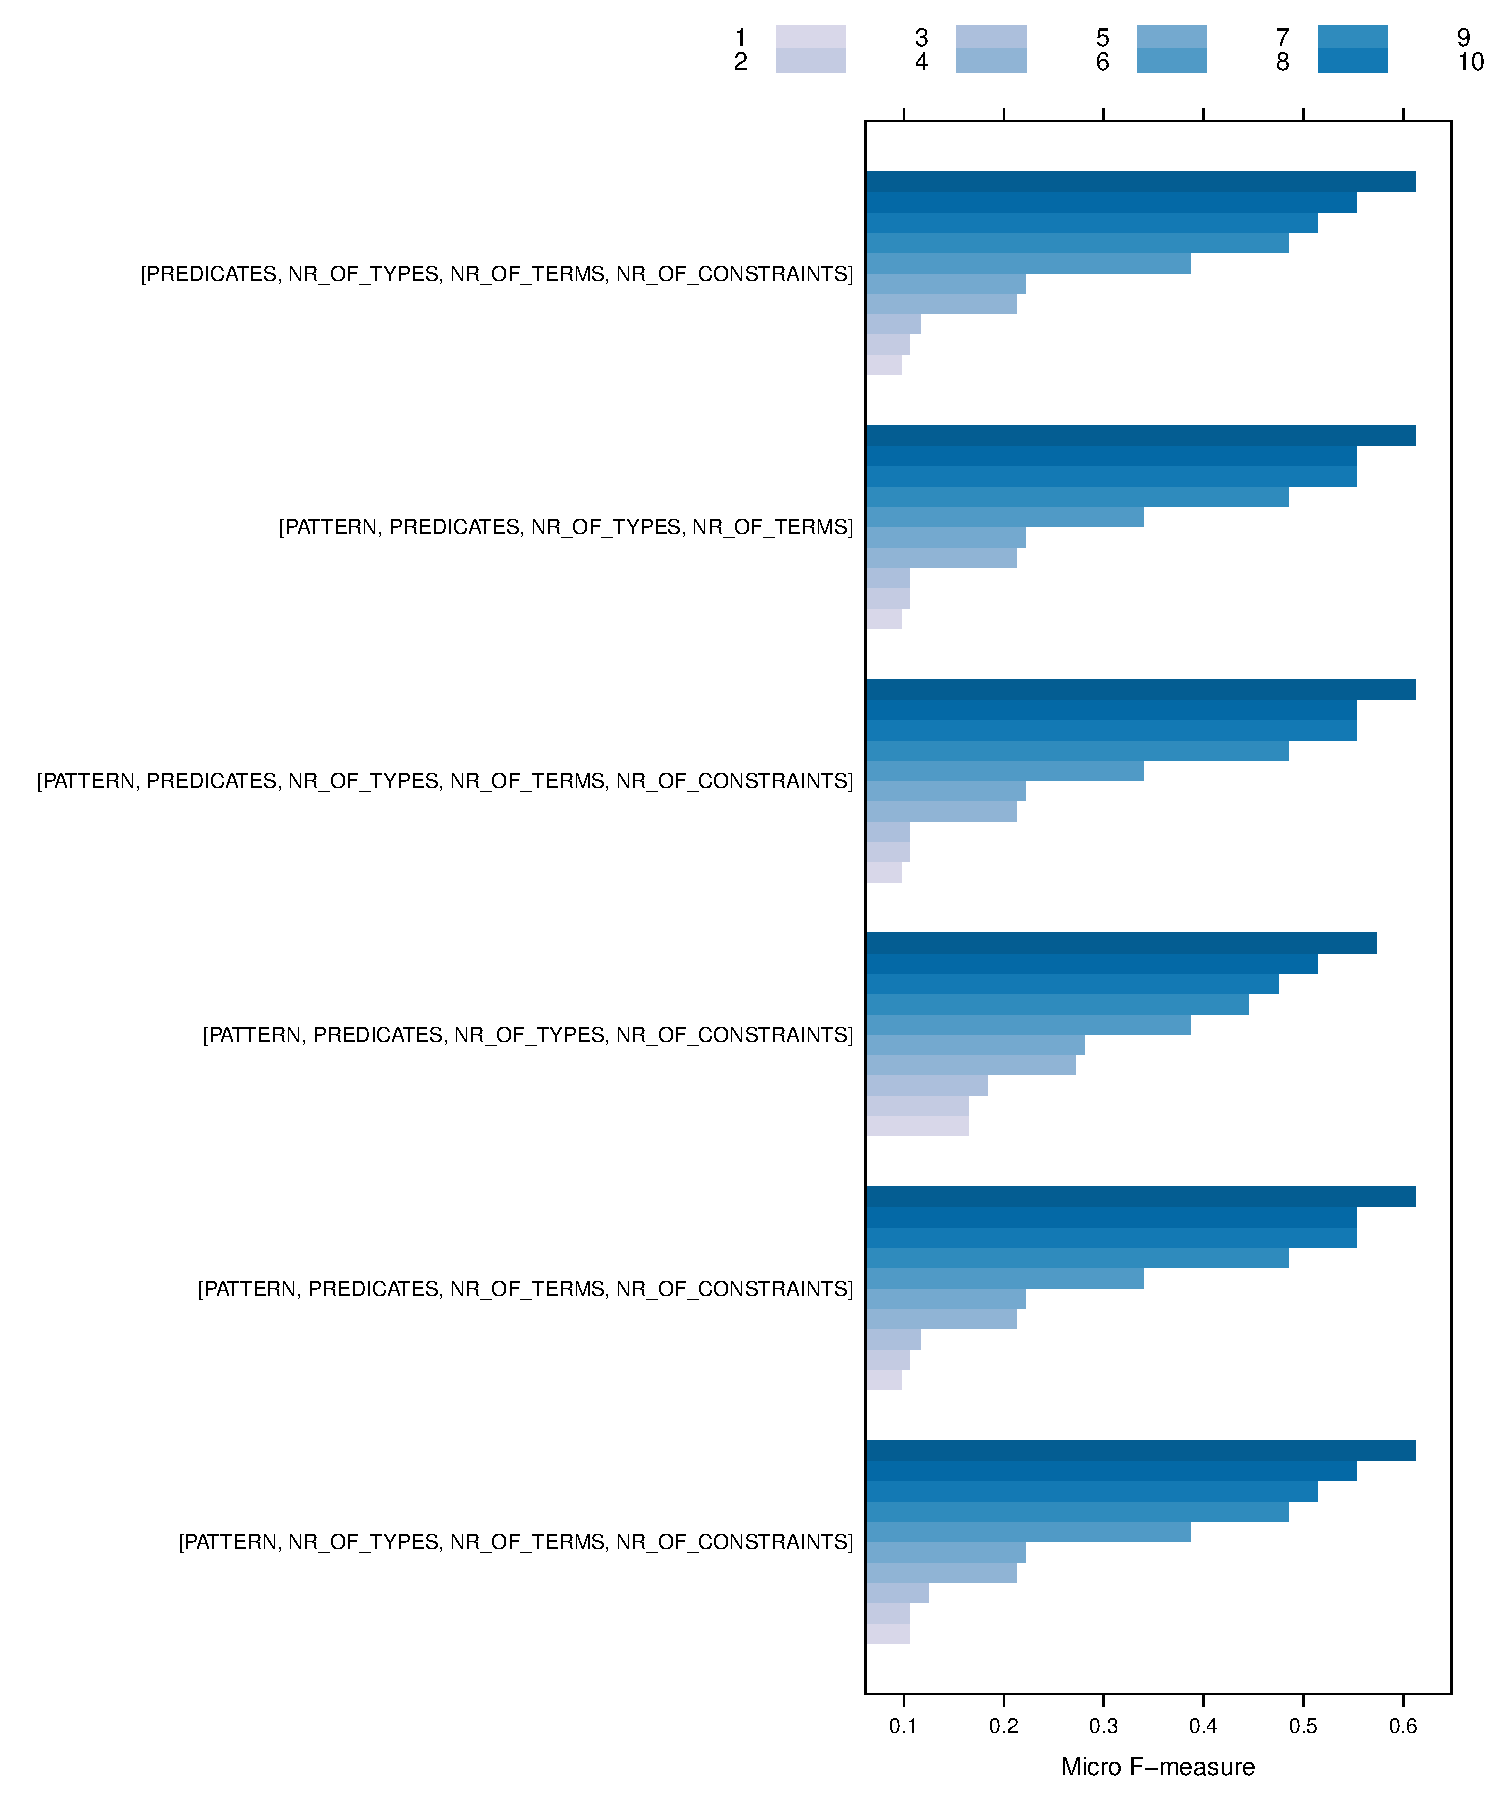
\includegraphics[width=\linewidth]{ranking_45}
%\captionof{figure}{F-measures on training dataset using $N=[1,\ldots,10]$ and using four and five features.}
%\label{chahawk:fig:ranking_45}
%\end{minipage}

Delving deeper into this analysis, we find:
\begin{itemize}
\item Although \textbf{NR\_OF\_TERMS} produces the largest sum of F-measures as a single feature, \textbf{NR\_OF\_CONSTRAINTS} achieves a higher F-measure as soon as $N=7$ due to the larger number of needed constraints with respect to the query length.
\item The highest mass of F-measure reaches the pair \textbf{PREDICATES, NR\_OF\_TERMS} with an F-measure of 0.58 at $N=10$. However, HAWK is able to achieve a higher F-measure of 0.61 at $N=10$ using \textbf{NR\_OF\_TERMS, NR\_OF\_CONSTRAINTS}.
\item We only regard the top-10-ranked queries. The correct queries belonged to the top-n queries as shown in Table~\ref{tab:trainqueries}.
\item The combination of three or all four features does not lead to an improvement. % of the F-measure. 
\end{itemize}

HAWK generates up to 15000 SPARQL queries per question containing more than one query generating the correct answer. 
%\todo[inline]{elaborate}
We consider ranking the resulting SPARQL queries most challenging with respect to the fact that an ideal ranking can lead to F-measures up to 0.72 at $N=1$.
%\todo[inline]{@Axel: does that make sense here: show graph where queries with expected several entities in the answer have LIMIT N against F-measure}

\subsection{Error Analysis}

In the following, we analyze error sources in HAWK based on the training queries failing to reach a higher F-measure.
Table~\ref{tab:trainqueries} shows for each entity search question from the training dataset its evaluation results.
\begin{itemize}
\item \textbf{Entity Annotation: } Queries 1, 11 and 15 cannot be answered by HAWK due to failing entity annotation. None of the tested annotation tools was able to either find the resources  \texttt{Jane\_T.\_Austion} nor \texttt{G8} or \texttt{Los\_Alamos}. 
Without matching entity annotations a full-text search retrieves too many matches for reaching high precision values on limited result set.
\item \textbf{Missing type information:} some of the resources of the gold standard do not have appropriate type information leading to a high amount of queries that need to be ranked correctly.
\item \textbf{Query structure: } Queries like 11 or 15 inherit complex query structures leading to a multitude of interpretations while generating the SPARQL query graph.
\end{itemize}

%% Please add the following required packages to your document preamble:
% \usepackage{booktabs}
% \usepackage[table,xcdraw]{xcolor}
% If you use beamer only pass "xcolor=table" option, i.e. \documentclass[xcolor=table]{beamer}
\begin{table}[htb!]

 \resizebox{\textwidth}{!}{
\begin{tabular}{@{\extracolsep{\fill} } @{}lp{0.55\linewidth}lll@{}}
\toprule
\textbf{ID} & \textbf{Question}                                                                                 & \textbf{F-measure} & \textbf{Precision} & \textbf{Recall} \\ \midrule
\rowcolor[HTML]{FFCCC9} 
1           & Give me the currencies of all G8 countries.                                                       & 0.0                & 0.0                & 0.0             \\
2           & In which city was the assassin of Martin Luther King born?                                        & 1.0                & 1.0                & 1.0             \\
3           & Which anti-apartheid activist graduated from the University of South Africa?                      & 1.0                & 1.0                & 1.0             \\
\rowcolor[HTML]{BBDAFF} 
5           & Which recipients of the Victoria Cross died in the Battle of Arnhem?                              & 0.8                & 0.67               & 1.0             \\
6           & Where did the first man in space die?                                                             & 1.0                & 1.0                & 1.0             \\
\rowcolor[HTML]{BBDAFF} 
8           & Which members of the Wu-Tang Clan took their stage name from a movie?                             & 0.31               & 0.18               & 1.0             \\
\rowcolor[HTML]{BBDAFF} 
9           & Which writers had influenced the philosopher that refused a Nobel Prize?                          & 0.71               & 0.56               & 1.0             \\
\rowcolor[HTML]{FFCCC9} 
11          & Who composed the music for the film that depicts the early life of Jane Austin?                   & 0.0                & 0.0                & 0.0             \\
14          & Which horses did The Long Fellow ride?                                                            & 1.0                & 1.0                & 1.0             \\
\rowcolor[HTML]{9AFF99} 
15          & Of the people that died of radiation in Los Alamos, whose death was an accident?                  & 0.67               & 1.0                & 0.5             \\
\rowcolor[HTML]{BBDAFF} 
16          & Which buildings owned by the crown overlook the North Sea?                                        & 0.25               & 0.14               & 1.0             \\
\rowcolor[HTML]{BBDAFF} 
17          & Which buildings in art deco style did Shreve, Lamb and Harmon design?                             & 0.5                & 0.33               & 1.0             \\
18          & Which birds are protected under the National Parks and Wildlife Act?                              & 1.0                & 1.0                & 1.0             \\
19          & Which country did the first known photographer of snowflakes come from?                           & 1.0                & 1.0                & 1.0             \\
20          & List all the battles fought by the lover of Cleopatra.                                            & 1.0                & 1.0                & 1.0             \\
22          & Which actress starring in the TV series Friends owns the production company Coquette Productions? & 1.0                & 1.0                & 1.0             \\
23          & Dakar is the capital of which country member of the African Union?                                & 1.0                & 1.0                & 1.0             \\ \bottomrule
\end{tabular}}
\caption[QALD 4 training set performance.]{Micro measures: Precision=0.70 Recall=0.85 F-measure=0.72 at 17 queries from QALD 4 training set. Red indicates inability to generate correct query, Blue indicates missing precision and green missing recall.}
\label{tab:trainqueries}

\end{table}
\section{Related Work} 
\label{chahawk:sec:relatedwork}
Hybrid question answering is related to the fields of hybrid search and question answering over structured data. In the following, we thus give a brief overview of the state of the art in these two areas of research.

First, we present hybrid search approaches which use a combination of structured as well as unstructured data to satisfy an user's information need. 
Semplore~\cite{Zhang:2007a} is the first known hybrid search engine by IBM.
It combines existing information retrieval index structures and functions to index RDF data as well as textual data. 
Semplore focuses on scalable algorithms and is evaluated on an early QALD dataset.
Bhagdev et al.~\cite{Bhagdev:2008:HSE} describe an approach to hybrid search combining keyword searches, Semantic Web inferencing and querying. 
The proposed K-Search outperforms both keyword search and pure semantic search strategies.
Additionally, an user study reveals the acceptance of the Hybrid Search paradigm by end users.
%K-Search retrieves only documents where a full-text match and an ontology match via SPARQL is available, loosing possible matching documents.
%Results achieved with K-Search are not replicable because of the closed nature of the underlying data.
%Especially, the authors point out the importance of keywords-in-context queries. 
%For example, semantic search can only deliver which component of an engine is located on or nearby another. 
%A full text search will reveal which part of an engine broke at a certain event. 
%But with a keyword-in-context search you can derive which greater parts are affected or which common producer all parts have.
%Unfortunately, the paper lacks of formalisation and implementation details, neither an online demo is available.
%K-Search follows a formula-based search and hence exacerbate the input of arbitrary queries for all kinds of users.
%K-Search is a simple combination of IE and set operations over documents and triples enabling HS.
A personalized hybrid search implementing a  hotel search service as use case is presented in~\cite{DBLP:journals/kbs/Yoo12}. 
%An question- and answer-based system to infer the users personal preferences is introduced. 
By combining rule-based personal knowledge inference over subjective data, such as expensive locations, and reasoning, the personalized hybrid search has been proven to return a smaller amount of data thus resulting in more precise answers. 
%Additionally, Yoo presents an architectures for hybrid search and a novel hotel ontology derived from crowd data. 
Unfortunately, the paper does not present any qualitative evaluation and it lacks source code and test data for reproducibility. 
%Donghee Yoo presented in 2012 a personalized hybrid search~\cite{DBLP:journals/kbs/Yoo12} and implemented a personalized, hotel search service as use case.
%The author distinguishes between frequently updated and static data to choose whether to use query rewriting or query reasoning. 
%Moreover, an question-- and answer--based system to infer the users personal preferences is introduced. 
%By combining rule-based personal knowledge inference over subjective data (e.g. \emph{cheap hotels}) and reasoning over non-frequently changed datasets the personalized hybrid search has been proven to return a smaller amount of data claimed to be more precise.
%Unfortunately, the paper does not present any qualitative evaluation and it lacks source code and test data for reproducibility. 
All presented approaches fail to answer natural-language questions.
Besides keyword-based search queries, some search engines already understand natural language questions. Question answering is more difficult than keyword-based searches since retrieval algorithms need to understand complex grammatical constructs.
% thus impede speech input and conversational opportunities. 

%Using the whole available knowledge in the Web of Data requires queries to run simultaneously on a large number of stores. Providing federated search algorithms is a key technology to leverage real-time QA systems. (Nikolov et al. 2013) present a federated SPARQL search engine - FedSearch - which provides a hybrid combination of SPARQL and a full-text search tackling data heterogeneity . FedSearch is able to execute top-k search. Their vendor independent approach of full text search outperforms the state of the art in federated querying.
%\todo[inline]{Is there a benchmark for federated queries over Linked Data?}
%\todo[inline]{Benchmark data is not available anymore: http://wiki.aksw.org/projects/lodquery}
%\todo[inline]{SINA does not work. Make sure Hydra works all the time}
%\subsection{Question Answering}
Second, we explain several QA approaches in the following.
{Schlaefer et al.~\cite{ephyra2007}} describe \emph{Ephyra}, an open-source question answering system and its extension with factoid and list questions via semantic technologies.
%Using semantic technology like Wordnet as well as a answer type classifier to combine statistical, fuzzy models and previously developed, manually refined rules.
%\todo[inline]{Instead of their hand-coded answer-type-hierarchy, we could make use of relations extracted from ontologies.The authors use a AdaBoost based classifier for answer merging}
Using Wordnet as well as an answer type classifier to combine statistical, fuzzy models and previously developed, manually refined rules. The disadvantage of this system lies in the hand-coded answer type hierarchy. % which prohibits its multi-lingual use.
%Ephyra is an open source QA system presented by (Schlaefer et al., 2007). It is able to deal with standard natural language questions as well as with factoid and list questions via semantic technologies. 
Cimiano et al.~\cite{orakel} developed \emph{ORAKEL} to work on structured knowledge bases.
The system is capable of adjusting its natural language interface using a refinement process on unanswered questions. 
Using F-logic and SPARQL as transformation objects for natural language user queries it fails to make use of Semantic Web technologies such entity disambiguation.
{Lopez et al.~\cite{poweraqua}} introduce \emph{PowerAqua}, another open source system, which is agnostic of the underlying yet heterogeneous sets of knowledge bases. 
It detects on-the-fly the needed ontologies to answer a certain question, maps the users query to Semantic Web vocabulary and composes the retrieved (fragment-)information to an answer. However, PowerAqua is outperformed by TBSL (see below) in terms of accuracy w.r.t. the state-of-the-art QALD 3 benchmark.
{Damljanovic et al.~\cite{freya}} present \emph{FREyA} to tackle ambiguity problems when using natural language interfaces. 
Many ontologies in the Semantic Web contain hard to map relations, e.g., questions starting with 'How long$\ldots$' can be disambiguated to a time or a distance. 
By incorporating user feedback and syntactic analysis FREyA is able to learn the users query formulation preferences increasing the systems question answering precision. 
{Cabrio et al.~\cite{qakis}} present a demo of \emph{QAKiS}, an agnostic QA system grounded in ontology-relation matches. 
The relation matches are based on surface forms extracted from Wikipedia to enforce a wide variety of context matches, e.g., a relation birthplace(person, place) can be explicated by X was born in Y or Y is the birthplace of X. 
Unfortunately, QAKiS matches only one relation per query and moreover relies on basic heuristics which do not account for the variety of natural language in general.
{Unger et al.~\cite{pythia}} describe \emph{Pythia}, a question answering system based on two steps.
First, it uses a domain-independent representation of a query such as verbs, determiners and wh-words.
Second, Pythia is based on a domain-dependent, ontology-based interface to transform queries into F-logic.
%The system has been evaluated on the geosystem ontology\footnote{\url{ftp://ftp.cs.utexas.edu/pub/mooney/nl-ilp-data/geosystem/}} and 880 annotated questions reaching an F-measure of 73.3\%.
Unfortunately, Pythia does not scale for larger domains since manual mapping of ontology terms via LexInfo is required.
%\todo[inline]{Use http://www8.cs.umu.se/~mjm/pubs/nldb09a.pdf to categorize otgher approaches}
Moreover, Unger et al.~\cite{tbsl} present a manually curated, template-based approach, dubbed \emph{TBSL}, to match a question against a specific SPARQL query. 
Combining natural language processing capabilities with Linked Data leads to good benchmark results on the QALD-3 benchmark (see below).
TBSL cannot be used to a wider variety of natural language questions due to its limited repertoire of 22 templates.
{Shekarpour et al.~\cite{SINA_WebSemantic}} develop \emph{SINA} a keyword and natural language query search engine which is aware of the underlying semantics of a keyword query. 
The system is based on Hidden Markov Models for choosing the correct dataset to query.
%Underlying is a SPARQL generation process which means SINA is only capable of dealing with Linked Data and cannot benefit from the wealth of unstructured information in the current Web.
%Due to the costly Hidden Markov Models SINAs answer time (on average 3.9s) is above enduser expectations.
%$(Shekarpour et al.,2013) introduce SINA a keyword and natural language query search engine which is aware of the underlying semantics of a keyword query. Based on Hidden Markov Models for choosing the correct dataset to query and a underlying  SPARQL generation process enables SINA to benefit from Linked Data. So far SINA is not capable of working with unstructured information and time inefficient as well.
%HMM is a very costly algorithm which can be substituted by a tuned dynamic programming algorithm tuned with a larger number of logs.
%SINA needs at leas 3.9s to answer a question which is unacceptable since users do not wait for more than 1s until they want to see the SERP.
\emph{Treo}~\cite{treo} emphasis the connection between the semantic matching of input queries and the semantic distributions underlying knowledge bases.
The tool provides an entity search, a semantic relatedness measure, and a search based on spreading activation.
Recently, Peng et al.~\cite{DBLP:journals/corr/PengZZ14} describe an approach for hybrid QA mapping keywords as well as resource candidates to modified SPARQL queries. 
Due to its novelty we were not able to compare it to HAWK.

Several industry-driven QA-related projects have emerged over the last years. 
For example, DeepQA of IBM Watson~\cite{watson}, which was able to win the Jeopardy! challenge against human experts. 
%The results of this project are yet not open-source and are thus of limited use for the QA community. 
%Moreover, the Watson API is restricted to only a few users. 
Further, {KAIST's Exobrain\footnote{\url{http://exobrain.kr/}}} project aims to learn from large amounts of data while ensuring a natural interaction with end users. 
However, it is yet limited to Korean for the moment. % and does not aim to enable an open-source access to its components.

The field HAWK refers to is hybrid question answering for the Semantic Web, i.e., QA based on hybrid data (RDF and textual data).
To the best of our knowledge, none of the previous works has addressed this question so far.
%\todo[inline]{ On The Marriage of SPARQL and Keywords
%  by Peng Peng, Lei Zou, Dongyan Zhao
%* Semplore: An IR Approach to Scalable Hybrid Query of Semantic Web Data
%  byLei Zhang, QiaoLing Liu, JieZhang, HaoFen Wang, Yue Pan, Yong Yu
%   Venses is hybrid in the sense that it combines different rule systems while the second paper simply combines different algorithms on text (QA4MRE data).
%  * VENSES GetAsk: a System for Hybrid Question Answering And Answer Recovery using Text Entailment
%•	A Hybrid Question Answering System based on Information Retrieval and Answer Validation}
%Lukovnikov presents~\cite{SESSA} a novel spread-activation-based entity search tool. 
%SESSA disambiguates and segments user input keyword queries using n-gram hierachies which are then the starting points for a coloured spread-activation algorithm. 
%This approach is the state of the art with respect to the QALD-3 entity-search benchmark with 56,9\% F-measure.
%In~\cite{fedsearch} a federated SPARQL search engine--FedSearch-- is presented. 
%Especially, the authors present a hybrid combination of SPARQL an full-text search tackling data heterogeneity and lacking statistical data.
%Their system is able to execute top-k search.
%Since SPARQL lacks full-text search support the authors propose a triple-store-independent way of querying different RDF stores such as OWLIM, Virtuoso and LuceneSail.
%Their vendor independent approach of keyword query search pattern is evaluated next to several optimizations against two benchmarks showing superior performs against other state-of-the-art systems-
For further insights please refer to~\cite{Kolomiyets:2011,DBLP:journals/semweb/LopezUSM11} which present surveys on existing question answering approaches.


\section{Conclusion}
\label{chahawk:sec:conclusion}
In this paper, we presented HAWK, the first hybrid QA system for the Web of Data. We showed that by using a generic approach to generate SPARQL queries out of predicate-argument structures, HAWK is able to achieve up to 0.68 F-measure on the QALD-4 benchmark. Our work on HAWK however also revealed several open research questions, of which the most important lies in finding the correct ranking approach to map a predicate-argument tree to a possible interpretation. So far, our experiments reveal that the mere finding of the right features for this endeavor remains a challenging problem. We thus aim to apply an automatic feature engineering approach from deep learning in future works to automatically generate the correct ranking function. Moreover, we aim to integrate HAWK in domain-specific information systems where the more specialized context will most probably lead to higher F-measures. Additionally, we will assess the impact of full-text components over regular LD components for QA, partake in the creation of larger benchmarks (we are working on QALD-5) and aim towards multilingual, schema-agnostic queries. Negations within questions and improved ranking will also be considered. Finally, several components of the HAWK pipeline are computationally very complex. Finding more time-efficient algorithms for these steps will be addressed in future works.
%\todo[inline]{HAWK considers SELECT queries and generate queries without UNION or OPTIONAL but we are aware of their advantages.}

